\documentclass[conference]{IEEEtran}
\usepackage[utf8]{inputenc}
\usepackage{amsmath,amssymb,amsfonts}
\usepackage{graphicx}
\usepackage{cite}
\usepackage{hyperref}
\usepackage{url}
\usepackage{balance}

\title{Mobile Device GNSS Spoofing Detection}

\author{
 \IEEEauthorblockN{Nathan Johnson}
 \IEEEauthorblockA{
    Embry-Riddle Aeronautical University\\
    Prescott, Arizona, USA\\
    johnsn63@my.erau.edu
  }
}

\begin{document}

\maketitle

\begin{abstract}
Global Navigation Satellite Systems (GNSS) play a critical role in modern infrastructure, from aviation and maritime navigation to time synchronization for cryptographic systems. However, the increasing reliance on GNSS has made it a valuable target for cyber threat actors, particularly through GNSS spoofing attacks. Unlike jamming, which simply disrupts GNSS signals, spoofing can deceive systems into using false positional data, leading to potentially severe consequences. This paper explores a novel approach to GNSS spoofing detection using mobile devices, leveraging onboard GNSS receivers and inertial sensors. Initial findings reveal significant limitations in consumer-grade accelerometers and gyroscopes for implementing a full Inertial Navigation System (INS). However, a simpler detection method based on monitoring deviations in GNSS position over time was developed. While this approach shows promise, false positive detections due to inherent GPS inaccuracies remain a challenge. Future work will focus on refining detection methods, potentially incorporating machine learning and noise reduction techniques to improve reliability.
\end{abstract}

\begin{IEEEkeywords}
GNSS, GPS spoofing, mobile security, inertial navigation system, cybersecurity, Android, sensor fusion, machine learning
\end{IEEEkeywords}
  

\section{Introduction}
Global Navigation Satellite Systems (GNSS) are an invisible and often overlooked yet critical piece of infrastructure. Many aspects of modern life rely on GNSS systems like the American GPS constellation or other systems like the Russian GLONASS constellation, EU Galileo constellation, or Chinese BeiDou constellation. GNSS systems fall under the broader category Position Navigation and Timing (PNT) systems which are used for military, aviation, maritime, and civilian navigation, but also for some unexpected purposes like synchronizing clocks around the world which plays a critical role in synchronizing the internet as well as time based cryptographic systems\cite{lu2021}. GPS based navigation in aviation is quickly making ground based forms of navigation obsolete due to its high flexibility and lower cost of implementation and maintenance. It is very common now for aircraft in instrument flight conditions, to be relying solely on the GPS system for navigation. Accurate GNSS service has also become critical for performing basic flight functions and stabilization in modern drones\cite{meng2021}.

As GNSS systems become more relied upon, their value as potential targets for cyber threat actors also grows. In recent years, GNSS jamming and spoofing attacks have become more and more prevalent, especially in areas with high geopolitical tension such as Ukraine and Iran.

GNSS jamming is a very simple form of denial of service attack involving the use of a radio transmitter to overpower the GNSS signals with noise. This is very easy to do as the frequencies which GNSS systems operate on are very well known and the satellites’ signals are very weak since they are being sent all the way from space.

GNSS jamming, however, is not nearly as big of a threat as GNSS spoofing. This is because it is extremely easy for systems to detect a total loss of GNSS signal and to gracefully fail over to a backup system. In the case of GNSS spoofing, a threat actor will overpower the legitimate GNSS satellites by transmitting false signals impersonating satellites. If done properly, the transition from real to spoofed GNSS signals can be extremely difficult to detect, leading systems to falsely trust and continue to operate using data being fed in from a malicious actor. Most targeted GNSS spoofing attacks work by replaying the accurate GNSS signals and then gradually applying a deviation to prevent a sudden detectable jump in position.

Several approaches to GNSS spoofing detection have been proposed. Power level based detection methods use the signal strength to try and determine when satellite based signals are being overpowered by stronger terrestrial signals, but as attackers become more advanced and carefully tune their transmit power, this method is becoming more difficult to use. Most other methods of detection rely on a comparison of the received GNSS signals to some known good position information. This includes ground based stations at a known location checking for GPS error. Another method proposed for aviation and drones is to make use of the aircraft’s onboard accelerometers and gyroscopes. Almost all modern aircraft have an Inertial Navigation System (INS). This system operates using a known starting position and then continuously integrating extremely precise data from the accelerometers and gyroscopes to calculate how the aircraft’s position has changed over time. Due to the nature of these systems, they can only be used in isolation for a limited time before the accumulation of error renders them unreliable and they need to be periodically reset using GPS position. It is theoretically possible, however, to compare the relative velocities calculated by the INS and  GPS.\@ If an unusually high difference was noted, it could be evidence that spoofing is taking place\cite{meng2021}.

For my CI 515 project, I have decided to take advantage of mobile devices having both onboard GNSS receivers and accelerometers and gyroscopes to explore a possible implementation of this detection method.

\section{Related Work}
Several studies have been done assessing the effectiveness of GNSS spoofing detection by comparing GNSS position to inertial position, including a 2021 study utilizing the accelerometers and gyros onboard drones\cite{meng2021}. However, I am not aware of any studies that have attempted this technique using mobile devices.

\section{Tools and Methodology}
I have decided to implement my prototype mobile GNSS spoofing detection system in an android application. I am using Android Studio as my IDE and have been developing the app in Java as I have more experience in Java than Kotlin. I am currently developing using a Google Pixel 7 Pro and its onboard inertial systems and  GPS.\@ My initial approach was to try and implement a basic INS system in the app and then to compare the calculated latitude, longitude and altitude to what the GPS indicated. One of my fears going into this project is that the quality of the sensors in consumer mobile devices is not up to the same standard as those that are installed in aircraft and drones.

\begin{figure}[htbp]
 \centerline{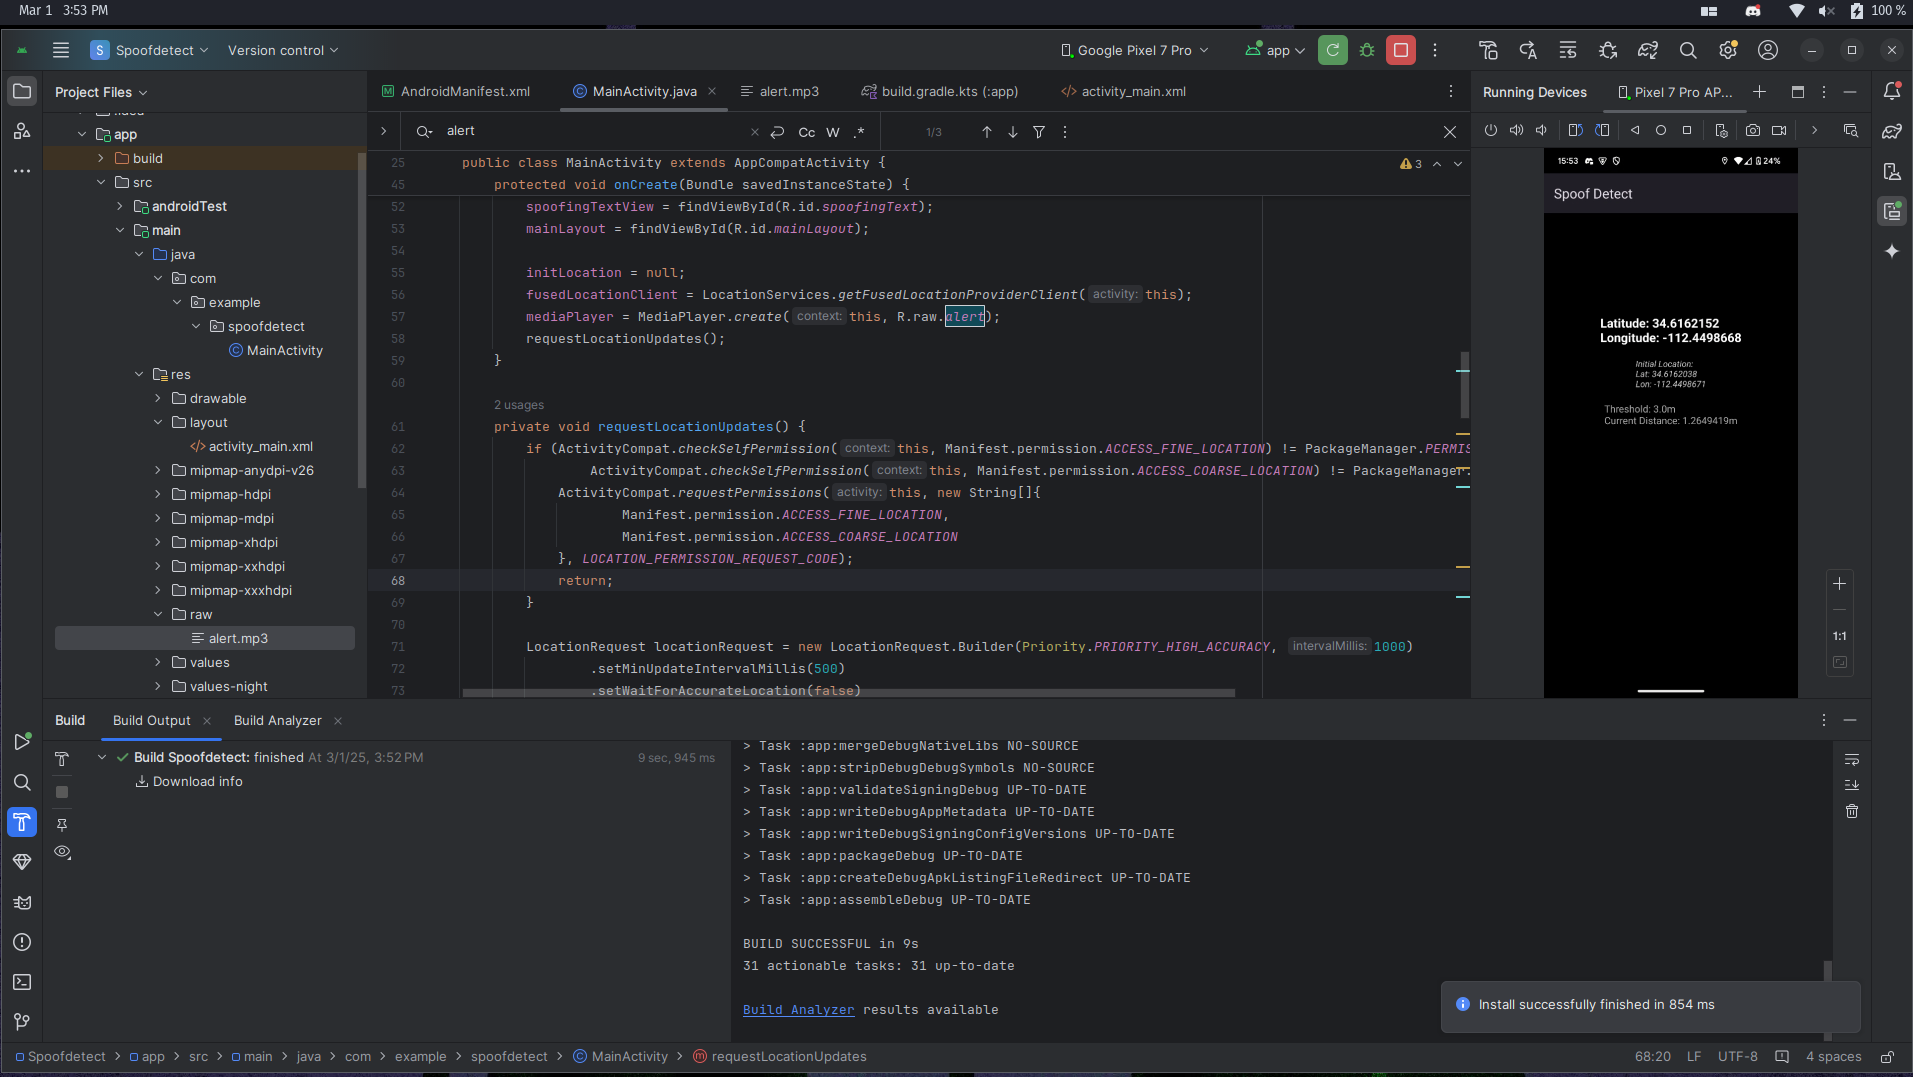
\includegraphics[width=0.5\textwidth]{figs/android_studio.png}}
 \caption{Screenshot of source code in Android Studio.}
\end{figure}

\section{Progress and Initial Findings}
So far, I have been unable to get accurate enough data from the phone’s sensors to be useful. The GPS position, which updates once per second, varies by several meters on each update, which is not terrible, but will make it impossible to detect very fine spoofing attacks. 

I have also determined that the phone’s accelerometers are nowhere near accurate enough to keep track of the phone’s position in real time. While I never fully implemented an INS, I did implement a basic test system for tracking the phone’s position. I aligned the phone face up along a North-south axis. I then used the phone’s x-y accelerometers. I performed numerical integration twice on the x and y acceleration to integrate from acceleration to velocity and then to position. This change in position was then added to the phone's running estimate of its latitude and longitude. It became immediately clear that inaccuracy of the accelerometers was accumulating rapidly, resulting in useless data. This was extremely disappointing, but I expected this to be the case.

My new strategy is to assume that the phone is to remain stationary. The current version of the app will first wait for the gps to acquire signal and then stabilize. It will then store this initial position and this will be trusted to be the phone's true position. The GPS position will then be checked every second and the distance between the measured position and the initial position is calculated. If the distance between these two measurements exceeds a set tolerance, currently 3 meters, the app will register a detection of GPS spoofing. Due to the inaccuracy of the consumer grade GPS receiver in the phone, this is still not effective. The measured position from the phone’s GPS varies widely within a range up to about 10 meters leading to many false positive detections. The accuracy does improve when taking the phone outdoors, but not by much.

\begin{figure}[htbp]
 \centerline{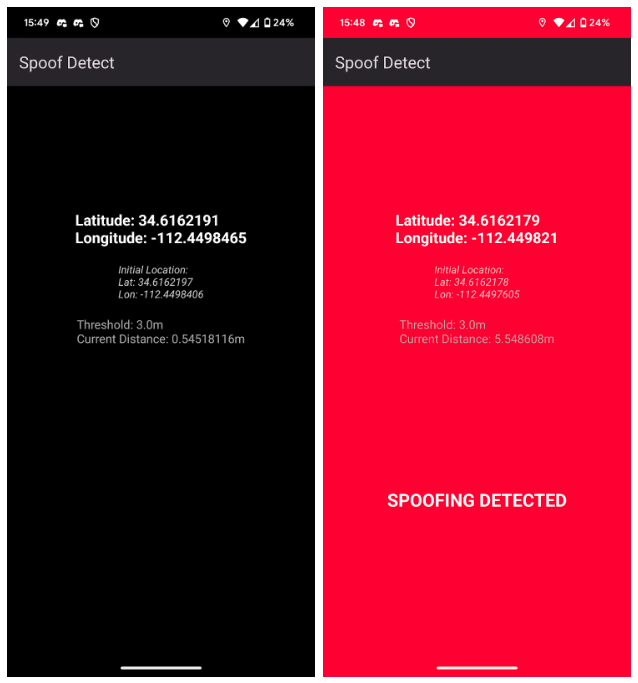
\includegraphics[width=0.5\textwidth]{figs/spoofdetect_app.png}}
 \caption{Screenshot of Spoofdetect Android app.}
\end{figure}

\section{Next Steps}
For the second half of this project, I would still like to create a functional GNSS spoofing detection system. I have not experimented with any machine learning models which may be a cool direction to go if there is time. I will definitely attempt to implement some type of noise reduction, such as keeping a moving average of the GPS position rather than the raw sensor data.

\section{Conclusion}
The investigation into GNSS spoofing detection using mobile devices has demonstrated both the potential and limitations of consumer-grade hardware for this application. While initial attempts to implement an inertial navigation-based detection system proved infeasible due to sensor inaccuracies, an alternative method using position deviation tracking was developed. The primary challenge remains the inherent imprecision of mobile GPS receivers, leading to false positive detections. Moving forward, the implementation of noise reduction techniques, such as moving averages, may help refine detection accuracy. Additionally, incorporating machine learning to identify spoofing patterns could further enhance reliability. As GNSS spoofing continues to grow as a cybersecurity threat, developing accessible and effective detection methods remains an important pursuit.

\nocite{*}
\bibliographystyle{IEEEtran}
\bibliography{references}

\balance{}

\end{document}